%--------------------------------------------------------------------
%--------------------------------------------------------------------
% Formato para los talleres del curso de Herramientas Computacionales
% Universidad de los Andes
%--------------------------------------------------------------------
%--------------------------------------------------------------------

\documentclass[12pt,letterpaper]{exam}
\usepackage[utf8]{inputenc}
\usepackage[spanish]{babel}
\usepackage{graphicx}
\usepackage{mdframed}
\usepackage[absolute]{textpos} 
\mdfdefinestyle{mystyle}{leftmargin=1cm,rightmargin=1cm,linecolor=blue}

\newcommand{\base}[1]{\underline{\hspace{#1}}}
\boxedpoints
\pointname{ pt}
%\extrawidth{0.75in}
%\extrafootheight{-0.5in}
%\extraheadheight{-0.25in}
%\pagestyle{head}

\noprintanswers
%\printanswers
\renewcommand{\solutiontitle}{}
\SolutionEmphasis{\color{blue}}

\begin{document}
\begin{center}
{\Large Herramientas Computacionales} \\
Taller 2 - \LaTeX (1) \\
{\small \it Febrero de 2015}
\end{center}

\begin{textblock*}{40mm}(10mm,20mm)
  
\includegraphics[width=3cm]{logoUniandes.png}
\end{textblock*}

\begin{textblock*}{40mm}(161mm,20mm)
  
\includegraphics[width=3cm]{logoUniandes.png}
\end{textblock*}



Las respuestas a los ejercicios del 1 al 3 deben ser entregadas en un solo archivo de \LaTeX $\,$ nombrado con el formato \verb"NombreApellido_HW2-1.tex". El último ejercicio debe ser entregado en otro archivo nombrado con el formato \verb"NombreApellido_HW2-2.tex". Ambos archivos deben ser entregados a través de {\bf Sicua}.

\begin{questions}
\question Reproduzca en \LaTeX  las siguientes ecuaciones.
\begin{parts}
	\part[5] $\left(- \frac{\hbar^2}{2 m} \nabla^2 + V \right) |\psi\rangle = i \hbar \frac{d |\psi\rangle}{dt}$
%	\begin{EnvFullwidth}
	\begin{solution}
		\begin{verbatim}
		 $\left(- \frac{\hbar^2}{2 m} \nabla^2 + V \right) |\psi\rangle = 
		 i \hbar \frac{d |\psi\rangle}{dt}$
		\end{verbatim}
	\end{solution}
%	\end{EnvFullwidth}
	\part[5] $\sum_{n=1}^{\infty}{ \frac{1}{n^2} } = \frac{\pi^2}{6}$
	\begin{solution}
		\begin{verbatim}
			$\sum_{n=1}^{\infty}{ \frac{1}{n^2} } = \frac{\pi^2}{6}$
		\end{verbatim}
	\end{solution}
	\part[5] $\left(\beta mc^2 + c \left(\alpha_1 p_1 + \alpha_2 p_2 + \alpha_3 p_3\right)\right) \psi\left(x,t\right) = i \hbar \frac{\partial \psi\left(x,t\right)}{\partial t}$
	\begin{solution}
		\begin{verbatim}
			$\left(\beta mc^2 + c \left(\alpha_1 p_1 + \alpha_2 p_2 + 
			\alpha_3 p_3\right)\right) \psi\left(x,t\right) = 
			i \hbar \frac{\partial \psi\left(x,t\right)}{\partial t}$
		\end{verbatim}
	\end{solution}
	\part[5] $\int_{-\infty}^{\infty} e^{-\frac{x^2}{2\sigma^2}} \textrm{d}x = \sqrt{2\pi} \sigma$
	\begin{solution}
		\begin{verbatim}
			$\int_{-\infty}^{\infty} e^{-\frac{x^2}{2\sigma^2}} \textrm{d}x = 
			\sqrt{2\pi} \sigma$
		\end{verbatim}
	\end{solution}
	\part[5] $\frac{P}{A} = \frac{2\pi \left(k T\right)^4}{h^3 c^2} \int_{0}^{\infty} \frac{x^3}{e^{x}-1}\, \textrm{d}x = \frac{2\pi^5 k^4}{15 h^3 c^2}\,T^4$
	\begin{solution}
		\begin{verbatim}
			$\frac{P}{A} = \frac{2\pi \left(k T\right)^4}{h^3 c^2} 
			\int_{0}^{\infty} \frac{x^3}{e^{x}-1}\, \textrm{d}x 
			= \frac{2\pi^5 k^4}{15 h^3 c^2}\,T^4$
		\end{verbatim}
	\end{solution}
	\part[5] $\sum_{i}{ \vec{F}_i } = m \vec{a}$
	\begin{solution}
		\begin{verbatim}
			$\sum_{i}{ \vec{F}_i } = m \vec{a}$
		\end{verbatim}
	\end{solution}
	\part[5] $\left(
		\begin{array}{cc}
 			a & b \\
 			c & d \\
		\end{array}
		\right)^{-1} = \frac{1}{ad - bc}  \left(
		\begin{array}{cc}
 			d & -b \\
 			-c & a \\
		\end{array}
		\right)$
	\begin{solution}
		\begin{verbatim}
			$\left(
		\begin{array}{cc}
 			a & b \\
 			c & d \\
		\end{array}
		\right)^{-1} = \frac{1}{ad - bc}  \left(
		\begin{array}{cc}
 			d & -b \\
 			-c & a \\
		\end{array}
		\right)$
		\end{verbatim}
	\end{solution}
%	\part 	$\begin{tabular}{|c|c|}
%		\hline
% 		a & b \\
% 		\hline
% 		c & d \\
%		\hline
%	\end{tabular}$
%	\begin{solution}
%		\begin{verbatim}
%			$\begin{tabular}{|c|c|}
%		\hline
% 		a & b \\
% 		\hline
% 		c & d \\
%		\hline
%	\end{tabular}$
%		\end{verbatim}
%	\end{solution}
\end{parts}
	
\question[20] Reproduzca en \LaTeX el siguiente fragmento\footnote{Tomado de {\it Principles of Mathematical Analysis} de Walter Rudin.}: 
\begin{mdframed}[style=mystyle]
	\vspace{0.2cm}
	{\bf{6.1 Definition}} Let $\left[ a,b \right]$ be a given interval. By a {\it partition} $P$ of $\left[ a,b \right]$ we mean a finite set of points $x_0, x_1, \ldots, x_n$, where
	\[
		a = x_0 \le x_1 \le \ldots \le x_{n-1} \le x_n = b.
	\]
	We write
	\[
		\Delta x_i = x_i - x_{i-1}\,\,\,\, \left(i=1,\ldots,n\right).
	\]
	\vspace{0cm}
\end{mdframed}
	\begin{solution}
		\begin{verbatim}
			\bf{6.1 Definition}} Let $\left[ a,b \right]$ be a given interval. By 
			a {\it partition} $P$ of $\left[ a,b \right]$ we mean a finite set 
			of points	$x_0, x_1, \ldots, x_n$, where
			\[
				a = x_0 \le x_1 \le \ldots \le x_{n-1} \le x_n = b.
			\]
			We write
			\[
				\Delta x_i = x_i - x_{i-1}\,\,\,\, \left(i=1,\ldots,n\right).
			\]
		\end{verbatim}
	\end{solution}

\question[20] Reproduzca lo siguiente usando los ambientes de alineación y formato adecuados:

\begin{flushleft}
	{\bf With fame I become more and more stupid, which \\
	of course is a very common phenomenon.} \\
	\underline {To Heinrich Zangger, December 24, 1919.}
\end{flushleft}
	
\begin{center}
	{\it With fame I become more and more stupid, which \\
	of course is a very common phenomenon.} \\
	{\footnotesize To Heinrich Zangger, December 24, 1919.}
\end{center}

\begin{flushright}
	\textsc{ With fame I become more and more stupid, which \\
	of course is a very common phenomenon.} \\
	{\footnotesize To Heinrich Zangger, December 24, 1919.}
\end{flushright}

\question[25] En el archivo adjunto están contenidos los cinco primeros capítulos de la primera parte del {\it Ingenioso hidalgo don Quijote de la Mancha} de Miguel de Cervantes, los títulos siendo los que se muestran a continuación.

	\begin{itemize}
		\item Capítulo Primero. De lo que el cura y el barbero pasaron con don Quijote cerca de su enfermedad
		\item Capítulo II. Que trata de la notable pendencia que Sancho Panza tuvo con la sobrina y ama de don Quijote, con otros sujetos graciosos
		\item Capítulo III. Del ridículo razonamiento que pasó entre don Quijote, Sancho Panza y el bachiller Sansón Carrasco
		\item Capítulo IV. Donde Sancho Panza satisface al bachiller Sansón Carrasco de sus dudas y preguntas, con otros sucesos dignos de saberse y de contarse
		\item Capítulo V. De la discreta y graciosa plática que pasó entre Sancho Panza y su mujer Teresa Panza, y otros sucesos dignos de felice recordación
	\end{itemize}

Construya un libro, que incluya título, tabla de contenidos, y el texto de estos cinco capítulos.

\vspace*{\fill}
\begin{center}
	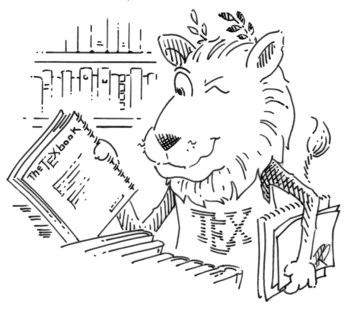
\includegraphics[width=0.6\textwidth]{./ctan_lion.png}
	
	{\it CTAN lion drawing by Duane Bibby}
\end{center}
\vspace*{\fill}

\end{questions}
\end{document}
